\documentclass[convert, tikz]{standalone}
%\usepackage{xcolor}
\begin{document}
%\pagecolor[RGB]{255,255,254}
  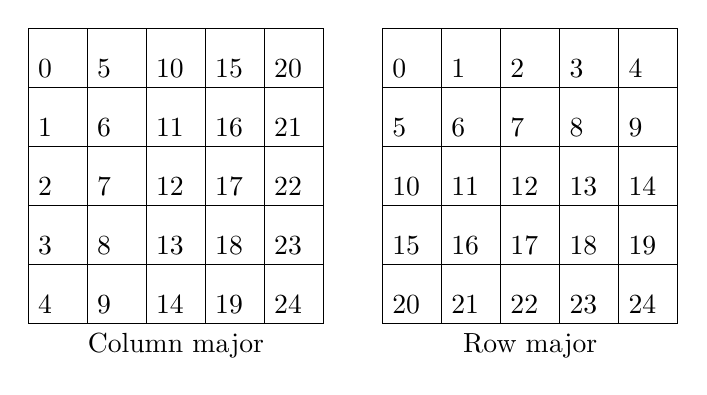
\begin{tikzpicture}[scale=0.75]
    \begin{scope}
      \draw(0,0) grid(5,5);
      \foreach \i in {0,...,4}{
        \foreach \j in {0,...,4}{
          \pgfmathsetmacro\idx{5*\i+4-\j}
          \node[above right] at (\i,\j) {\pgfmathprintnumber{\idx}};
        }
       }
      \node[below] at (2.5,0) {Column major};
    \end{scope}
    \begin{scope}[xshift=6cm]
      \draw(0,0) grid(5,5);
      \foreach \i in {0,...,4}{
        \foreach \j in {0,...,4}{
          \pgfmathsetmacro\idx{5*(4-\j)+\i}
          \node[above right] at (\i,\j) {\pgfmathprintnumber{\idx}};
        }
       }
      \node[below] at (2.5,0) {Row major};
    \end{scope}
  \end{tikzpicture}
\end{document}
